\documentclass[twocolumn]{aastex701}

\usepackage{amsmath}
\usepackage{amsthm}
\newtheorem{proposition}{Proposition}

\shorttitle{Stable area of three overlapping disks}
\shortauthors{Author}

\newcommand{\dth}{\Delta\theta}

\begin{document}

\title{The Common Overlap of Three Disks: an Exact, Backward-stable and Fast Solution for Mutual Transits and Eclipses}

\author{A. Author}
\affiliation{Institution}
\email[show]{author@example.org}

\begin{abstract}
The area common to three disks determines the light blocked during mutual
events of transiting planets, moons and eclipsing multiple stars. The
published closed forms are incomplete or incorrect: the formula of Fewell
and the light-curve code LUNA that adopted it fail whenever the overlap
contains more than half of one disk, a case later repaired by a dedicated
branch, and the textbook lens formula used for the lens topologies loses
all significant digits for thin overlaps. We present a new solution that
removes every case distinction from the evaluation. We prove that a
non-degenerate overlap has at most four corners, which reduces the
geometry to five topologies resolved by a single directed walk along the
boundary arcs. Green's theorem then yields the area as a sum of circular
segments and a vertex polygon whose evaluation requires one arctangent per
arc, contains no subtractive cancellation, and treats arcs longer than
$\pi$ without a special case. Against 50-digit references for $21{,}568$
configurations, including triangles of $10^{-15}$ times the smallest disk
and lenses of depth $10^{-7}$, the error never exceeds $2.01$ times the
condition number of the problem times the unit roundoff: the algorithm is
componentwise backward stable, whereas the classical formulas exceed this
bound by factors of up to $10^{16}$. Five public packages that compute
the same area, among them the mutual-transit code \texttt{gefera}, fail on
121 to $21{,}568$ of $40{,}000$ test configurations through undefined
values, missing topologies or lost precision; the present method fails on
none. The complete computation costs 45\,ns per configuration on one CPU
core, comparable to the bare closed form of a single topology and four to
several thousand times faster than the public packages.
The same decomposition delivers the centroid of the overlap in closed form.
An open-source implementation is available at
\url{https://github.com/hippke/reuleaux}.
\end{abstract}

\keywords{Exoplanets --- Transits --- Exomoons --- Eclipsing binary stars --- Computational methods}

\section{Introduction} \label{sec:intro}

When two bodies transit a star simultaneously and overlap on the sky, the
stellar light they block is the area of the union of their shadows on the
stellar disk. With the star, a planet and its moon represented by three
disks, the union follows from the pairwise lenses and one further
quantity, the area of the common overlap of all three disks. Mutual events
of this kind constrain the orbits of exomoons \citep{CabreraSchneider2007,
Kipping2011, HippkeHeller2022, Kalman2023}, planet--planet occultations
\citep{Luger2017} and multiply eclipsing stellar systems
\citep{Short2018}. The single-body occultation is solved analytically
\citep{MandelAgol2002, Agol2020, Luger2019}; the geometry of three disks
underlies every analytic treatment of the mutual case.

\citet{Fewell2006} gave the first closed form for the common overlap of
three circles. He decomposed the circular triangle into the straight
triangle on its three chords, evaluated with Heron's formula, and three
circular segments, and he classified the configurations into nine cases,
of which only one is a circular triangle. His expression for a segment
that exceeds half of its disk (his Eq.~16) retains the arcsine of the
chord, $r^2\arcsin(c/2r)$, which measures the minor arc, and omits the
term $\pi r^2$. \citet{Kipping2011} transcribed Fewell's construction to
the star--planet--moon problem in the algorithm LUNA, organised the
configurations into 27 principal cases with subcases, and inherited the
error in his Eq.~37 (case 14.1b). \citet{GordonAgol2022} identified the
discrepancy between LUNA and an exact computation near the inner edge of
the stellar limb and published the corrected segment,
$r^2[\pi-\arcsin(c/2r)] + (c/4)\sqrt{4r^2-c^2}$, in their Appendix~B. The
root cause is structural: a chord length determines an arc only up to the
choice between the arc and its complement, and every formula built on
chord lengths requires an additional geometric test to make that choice.

The exact limb-darkened light curve of two mutually transiting bodies
follows from Green's theorem, which converts the flux integral over the
visible stellar disk into line integrals along its boundary arcs
\citep{Pal2012}. \citet{GordonAgol2022} implemented this approach in the
code \texttt{gefera} with a tree of 16 geometric cases. Its published
Fortran returns undefined values when an intersection of the two
occulting bodies lies exactly on the stellar limb, and for a single body
when $b+r=1$, where the elliptic modulus reaches unity
(Section~\ref{sec:software}). \citet{Short2018} integrate the line integrals
numerically, \citet{Luger2017} discretise the star into annuli, and
\citet{Kalman2023} combine pixel classification with Gauss--Legendre
quadrature in the Transit and Light Curve Modeller \citep{Csizmadia2020}.
Outside astronomy, \citet{Librino2014} computed intersections of many
circles by inclusion--exclusion over a trellis of pairwise terms and
confirmed Fewell's construction as the reference for three circles.
Area-proportional Euler and Venn diagrams require the same quantity:
\texttt{eulerr} \citep{eulerr}, \texttt{venn.js} \citep{vennjs} and
\texttt{matplotlib-venn} \citep{mplvenn} compute intersections of circles
from their crossing points, polygon areas and circular segments, and
general geometry libraries such as Shapely \citep{shapely} on GEOS
\citep{geos} approximate disks by polygons. LUNA is not public.

All of these approaches rest on the area of a two-disk lens. Its textbook
form \citep{Weisstein},
\begin{equation}
\begin{split}
L ={}& r_1^2\arccos\frac{d^2+r_1^2-r_2^2}{2dr_1}\\
&+ r_2^2\arccos\frac{d^2+r_2^2-r_1^2}{2dr_2} - \tfrac12\sqrt{\Pi},
\end{split}
\label{eq:lens}
\end{equation}
with $\Pi=(-d+r_1+r_2)(d+r_1-r_2)(d-r_1+r_2)(d+r_1+r_2)$, subtracts
quantities of nearly equal size when the lens is thin, and the arccosine of
an argument $1-\epsilon$ amplifies the rounding error of the argument by
$\epsilon^{-1/2}$. For a small disk that barely enters a large one, the
regime of a moon at stellar ingress, Equation~(\ref{eq:lens}) loses every
significant digit (Section~\ref{sec:accuracy}). The same cancellation
affects the intersection points computed as $h^2=r_1^2-a^2$, which enter
all vertex-based formulas.

This paper presents a solution that is free of case-dependent formulas,
correct for arcs of any length, backward stable in floating-point
arithmetic, and as fast as the closed form of a single topology.
Section~\ref{sec:method} derives the method,
Section~\ref{sec:results} quantifies its accuracy and cost, and
Section~\ref{sec:discussion} discusses its scope.

\section{Method} \label{sec:method}

\subsection{Topology} \label{sec:topology}

Let $D_k$ denote the closed disk of centre $\mathbf{o}_k$ and radius $r_k$
bounded by the circle $C_k$, $k=0,1,2$, and let $R=D_0\cap D_1\cap D_2$.
If $D_i\subseteq D_j$ for some $i\neq j$, then $D_i\cap D_j=D_i$ and $D_j$
is removed; one remaining disk gives $A=\pi r^2$ and two give the lens of
the remaining pair. If any pair is disjoint, $A=0$. In the remaining
configurations every pair of circles crosses at two points. A crossing of
$C_i$ and $C_j$ that lies strictly inside $D_k$ is a vertex of $R$; let
$V$ be their number.

\begin{proposition}
If no crossing lies on the third circle, then $V\in\{0,2,3,4\}$. The
overlap is empty for $V=0$, the lens of one pair for $V=2$, a circular
triangle with one vertex from each pair for $V=3$, and a circular
quadrilateral whose four vertices lie on one circle for $V=4$.
\end{proposition}

\begin{proof}
$R$ is convex. If its interior is non-empty and $R$ is not a disk, its
boundary is a simple closed curve composed of $a_k$ arcs of each $C_k$,
joined at the vertices, so that $V=a_0+a_1+a_2$. An arc of $\partial R$ on
$C_i$ is a component of $(C_i\cap D_j)\cap(C_i\cap D_k)$, the intersection
of two proper arcs of $C_i$; hence $a_i\le2$, and $a_i=2$ holds exactly
when the two arcs cover $C_i$, i.e., $C_i\subset D_j\cup D_k$. Because
$D_j\cap D_k\neq\emptyset$, the union $D_j\cup D_k$ is simply connected,
and by the Jordan curve theorem it then contains $D_i$. A crossing
$\mathbf{q}$ of $C_j$ and $C_k$ lies on the boundary of $D_j\cup D_k$, so
$\mathbf{q}$ cannot lie in the interior of $D_i$: the pair $(j,k)$
contributes no vertex. Each vertex on $C_j$ then stems from the pair
$(i,j)$ and each on $C_k$ from $(i,k)$, which gives $a_j=a_k=1$ and $V=4$.
Otherwise $a_k\le1$ for all $k$ and $V\le3$. For $V=3$ every circle
carries one arc and two vertices; two vertices from the same pair would
leave the third circle without an arc, so each pair contributes one. For
$V=2$ the boundary consists of two arcs of the circles of one pair. A
boundary without vertices is a full circle $C_i\subset D_j\cap D_k$,
which the containment reduction has removed; therefore $V=0$ implies
$R=\emptyset$, and $V=1$ does not occur.
\end{proof}

The proposition replaces the 9, 27 and 16 cases of \citet{Fewell2006},
\citet{Kipping2011} and \citet{GordonAgol2022} by a count. Figure
\ref{fig:taxonomy} shows the five topologies.

\begin{figure*}
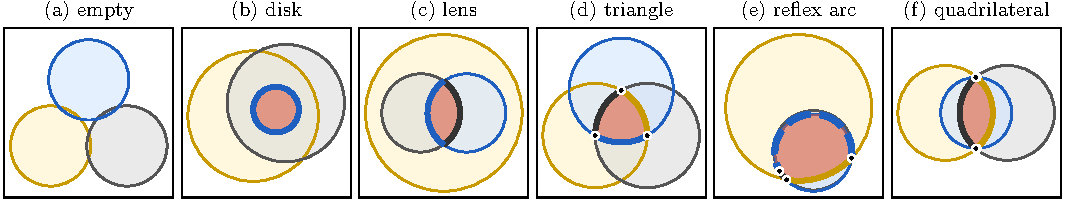
\includegraphics[width=\textwidth]{figures/taxonomy.pdf}
\caption{The topologies of the common overlap (red) of three disks after
containment reduction. Vertices are marked by dots, boundary arcs are
drawn in the colour of their circle, and the dashed arc in panel (e)
exceeds $\pi$. Panel (a) shows three pairwise intersecting disks without a
common point.}
\label{fig:taxonomy}
\end{figure*}

\subsection{Boundary walk} \label{sec:walk}

Traversed counter-clockwise, $\partial R$ runs counter-clockwise around
the centre of each of its arcs, because $R$ lies inside every disk. An arc
of $C_s$ between consecutive crossings on $C_s$ has constant membership in
the two other disks, and it belongs to $\partial R$ exactly when its
midpoint lies inside both. From every vertex $\mathbf{u}$ we therefore
select the unique counter-clockwise arc to another vertex $\mathbf{v}$ on
a shared circle $C_s$ whose open span contains no other crossing of $C_s$
and whose midpoint lies strictly inside the two other disks. With
$\mathbf{u}'=\mathbf{u}-\mathbf{o}_s$ and
$\mathbf{v}'=\mathbf{v}-\mathbf{o}_s$, the span test reduces to signs of
cross products, and the midpoint is
$\mathbf{o}_s\pm r_s(\mathbf{u}'+\mathbf{v}')/|\mathbf{u}'+\mathbf{v}'|$,
with the positive sign when $\mathbf{u}'\times\mathbf{v}'>0$. The
successors form a single cycle through all vertices; any other outcome
identifies a degenerate input. For $V=3$ each circle carries exactly two
vertices, the arcs follow the fixed adjacency of the three pairs, and the
midpoint test alone fixes their orientation. For $V=4$ the two arcs on the
circle that carries all vertices join angularly adjacent vertices in
counter-clockwise order. Both cases are evaluated without enumeration.

\subsection{Area} \label{sec:area}

Green's theorem gives $A=\frac12\oint(x\,dy-y\,dx)$. For the arc of $C_s$
from $\mathbf{u}$ to $\mathbf{v}$, parametrised as
$\mathbf{o}_s+r_s(\cos t,\sin t)$, the identities
$r_s(\sin\beta-\sin\alpha)=v_y-u_y$ and
$r_s(\cos\beta-\cos\alpha)=v_x-u_x$ remove all trigonometric functions of
the end angles:
\begin{equation}
A_{\rm arc}=\tfrac12\left[r_s^2\dth+o_{s,x}(v_y-u_y)-o_{s,y}(v_x-u_x)\right],
\label{eq:arc}
\end{equation}
\begin{equation}
\dth=\operatorname{atan2}\!\left(\mathbf{u}'\times\mathbf{v}',\,\mathbf{u}'\cdot\mathbf{v}'\right)\in(0,2\pi].
\label{eq:dtheta}
\end{equation}
Equation~(\ref{eq:dtheta}) determines the arc from the geometry rather
than from a chord length, so arcs longer than $\pi$ require no separate
treatment. Each term of Equation~(\ref{eq:arc}) equals the circular
segment of the arc plus the signed triangle
$(\mathbf{o}_s,\mathbf{u},\mathbf{v})$, and the triangle terms combine
around the cycle into the polygon of the vertices. The area therefore is
\begin{equation}
A=\sum_{\rm arcs}\frac{r_s^2}{2}\left(\dth-\sin\dth\right)
+\frac12\sum_{\rm edges}(\mathbf{u}-\mathbf{p})\times(\mathbf{v}-\mathbf{p}),
\label{eq:area}
\end{equation}
with $\mathbf{p}$ the first vertex. Equation~(\ref{eq:area}) generalises
the decomposition of \citet{Fewell2006} to every topology and every arc
length. It is evaluated in a form that contains no subtractive
cancellation beyond that inherent in the data. For $\dth<0.5$ the
segment uses the Taylor series
$\dth-\sin\dth=\sum_{n\ge1}(-1)^{n+1}\dth^{2n+1}/(2n+1)!$, truncated after
nine terms; for $\dth\ge0.5$ it uses
$r_s^2\sin\dth=\mathbf{u}'\times\mathbf{v}'$, which requires no further
transcendental function. The polygon is accumulated relative to
$\mathbf{p}$, so that its rounding error scales with the size of $R$ and
not with the coordinates. The input is translated to the centre of the
smallest disk. Figure~\ref{fig:method} illustrates the walk and the
decomposition.

\begin{figure*}
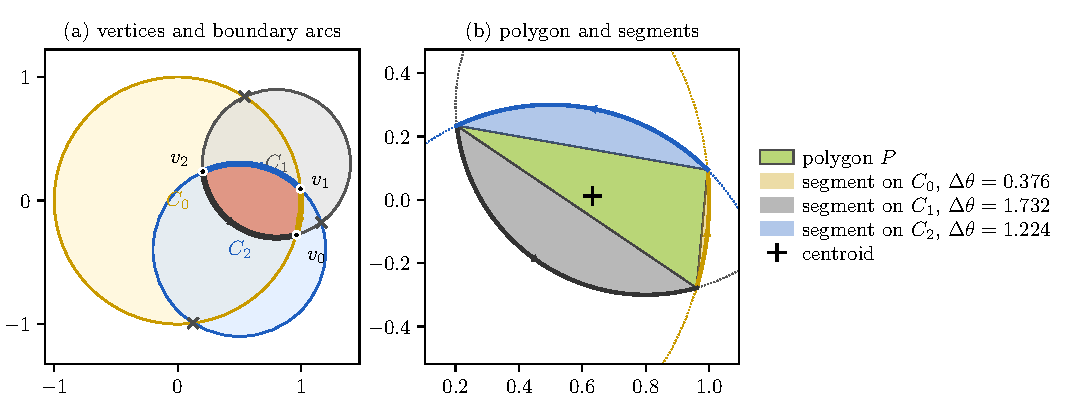
\includegraphics[width=\textwidth]{figures/method.pdf}
\caption{(a) Vertices of the overlap (dots), crossings outside the third
disk (crosses) and the directed boundary arcs. (b) Decomposition of
Equation~(\ref{eq:area}): vertex polygon and one circular segment per arc,
with the centroid of Equation~(\ref{eq:centroid}).}
\label{fig:method}
\end{figure*}

\subsection{Crossings and lenses} \label{sec:crossings}

The crossings of $C_1$ and $C_2$ at distance $d$ lie at distance
$a_1=[(d-r_2)(d+r_2)+r_1^2]/2d$ from $\mathbf{o}_1$ along the line of
centres and at distance $h$ from it, where $4d^2h^2$ is sixteen times the
squared area of the triangle with sides $(r_1,r_2,d)$. We evaluate it
with the ordering and bracketing of \citet{Kahan2014}: with
$\alpha\ge\beta\ge\gamma$ the sorted sides,
\begin{equation}
4d^2h^2=[\alpha+(\beta+\gamma)][\gamma-(\alpha-\beta)][\gamma+(\alpha-\beta)][\alpha+(\beta-\gamma)],
\label{eq:kahan}
\end{equation}
which retains full relative accuracy for needle-like triangles, i.e., for
nearly tangent circles. The lens follows from two segments with central
angles $2\operatorname{atan2}(h,a_1)$ and $2\operatorname{atan2}(h,a_2)$,
which replaces Equation~(\ref{eq:lens}).

\subsection{Degenerate input} \label{sec:degenerate}

Tangencies and containments within $10^{-12}$ of the largest radius
are resolved by the reduction of Section~\ref{sec:topology}. A crossing
within $10^{-9}$ of the third circle, a triple point, admits no reliable
inside test; the solution is then evaluated with all radii shifted by
$\pm10^{-8}$ of the largest radius and the two results are averaged. For a
circle through both corners of a lens the averaged area agrees with the
exact lens to $10^{-15}$, and for three circles through one point it
equals $7\times10^{-18}$.

\subsection{Centroid} \label{sec:centroid}

The decomposition of Equation~(\ref{eq:area}) yields the first moments of
$R$. The centroid of a segment with half-angle $\varphi=\dth/2$ lies on
its axis, beyond the chord midpoint by
\begin{equation}
\begin{split}
e&=r\left[\frac{4\sin^3\varphi}{3(2\varphi-\sin2\varphi)}-\cos\varphi\right]\\
&= r\left(\frac{\varphi^2}{5}-\frac{13\,\varphi^4}{1050}+\ldots\right),
\end{split}
\label{eq:centroid}
\end{equation}
and we evaluate the series, derived in exact rational arithmetic to order
$\varphi^{20}$, for $\varphi<0.5$. Together with the triangle fan of the
polygon this gives the centroid of the overlap to within $1.7\times10^{-12}$
of the smallest radius against an independent quadrature. The centroid
provides the first-order correction for the variation of the stellar
intensity across the overlap, which constant-intensity treatments of
mutual events omit.

\section{Results} \label{sec:results}

\subsection{Accuracy} \label{sec:accuracy}

We measure accuracy against references computed with 50 significant
digits \citep{mpmath}. The reference re-evaluates every vertex, angle,
segment and polygon of Equation~(\ref{eq:area}) in extended precision,
with the topology taken from the double-precision classification; that
classification agrees with an independent adaptive quadrature of the
chord length $\min_k(y_k+s_k)-\max_k(y_k-s_k)$, which contains no
geometric case logic, to $3.2\times10^{-14}$ of the smallest disk over
$20{,}000$ configurations. Five families sample the problem: general
disks, disks of similar radius with strong overlap, a hierarchical
star--planet--moon geometry with radii $1$, $0.02$--$0.2$ and
$0.005$--$0.1$, circular triangles produced by clipping a lens corner to
a depth of $10^{-7}$ to $0.5$ times the smallest radius, and thin lenses
of a small disk at the rim of a large one.

The attainable accuracy is limited by the conditioning of the problem. We
compute the componentwise relative condition number
$\kappa=\sum_i|p_i\,\partial A/\partial p_i|/A$ over the nine input
parameters by differentiation in extended precision. An algorithm whose
error does not exceed a small multiple of $\kappa u$, with
$u=2^{-53}$ the unit roundoff, returns the exact area of a configuration
perturbed by a few units of roundoff in its data and is backward stable
in the componentwise sense \citep{Higham2002}. Table~\ref{tab:accuracy}
and Figure~\ref{fig:accuracy} compare the present method with the direct
evaluation of Equation~(\ref{eq:arc}) using the textbook crossings and
Equation~(\ref{eq:lens}), with the corrected closed form of
\citet{Fewell2006} and \citet{GordonAgol2022} for circular triangles, and
with Equation~(\ref{eq:lens}) for lenses.

\begin{deluxetable*}{lrcccc}
\tablecaption{Maximum relative error and maximum error in units of $\kappa u$\label{tab:accuracy}}
\tablehead{
\colhead{Family} & \colhead{$N$} & \colhead{This work} & \colhead{Eq.~(\ref{eq:arc}), textbook} & \colhead{Eq.~(\ref{eq:lens})} & \colhead{Fewell + G\&A}
}
\startdata
general      & 2155 & $1.9\times10^{-13}$ / 1.1 & $2.0\times10^{-9}$ / $7.3\times10^{2}$ & $2.0\times10^{-9}$ / $7.3\times10^{2}$ & $1.5\times10^{-13}$ / 30 \\
similar      & 4995 & $1.4\times10^{-14}$ / 2.0 & $2.2\times10^{-13}$ / 5.8 & $4.2\times10^{-13}$ / 9.0 & $4.0\times10^{-14}$ / $1.3\times10^{2}$ \\
hierarchical & 4418 & $1.5\times10^{-12}$ / 1.3 & $2.1\times10^{-7}$ / $9.1\times10^{4}$ & $2.1\times10^{-7}$ / $9.1\times10^{4}$ & $3.4\times10^{-12}$ / $2.1\times10^{2}$ \\
corner       & 5000 & $9.9\times10^{-9}$ / 1.0 & $2.3\times10^{-2}$ / $1.1\times10^{6}$ & \nodata & $1.2\times10^{-8}$ / 1.4 \\
sliver lens  & 5000 & $1.5\times10^{-6}$ / 0.9 & $3.6\times10^{6}$ / $1.3\times10^{12}$ & $1.4\times10^{11}$ / $7.8\times10^{16}$ & \nodata \\
\enddata
\tablecomments{$N$ is the number of configurations with non-zero area.
Each entry gives the maximum relative error followed by the maximum of
the error divided by $\kappa u$. Equation~(\ref{eq:lens}) applies to
lens results, the closed form of \citet{Fewell2006} with the correction
of \citet{GordonAgol2022} to circular triangles.}
\end{deluxetable*}

\begin{figure*}
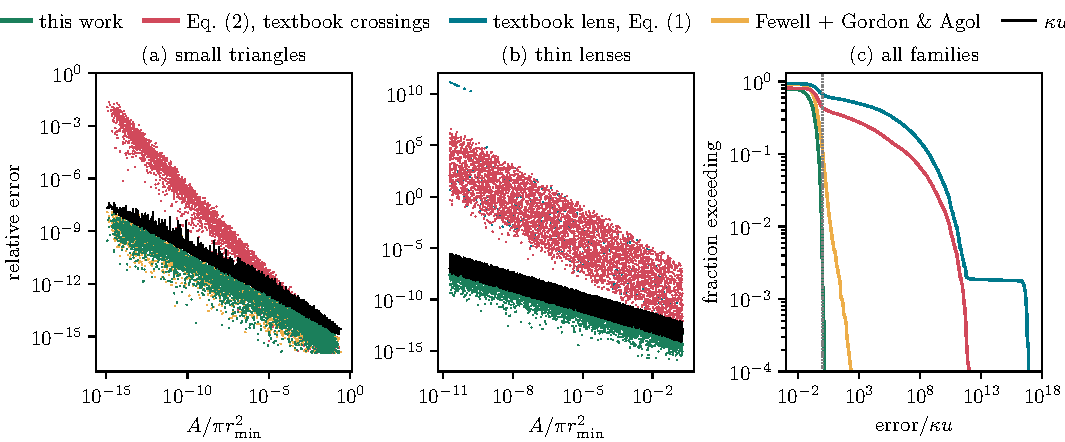
\includegraphics[width=\textwidth]{figures/accuracy.pdf}
\caption{Accuracy against 50-digit references. (a) Relative error of small
circular triangles versus their area in units of the smallest disk. (b)
Relative error of thin lenses. The black curve marks $\kappa u$. (c)
Fraction of all $21{,}568$ configurations whose error exceeds a given
multiple of $\kappa u$.}
\label{fig:accuracy}
\end{figure*}

The error of the present method never exceeds $2.01\,\kappa u$ in any of
the $21{,}568$ configurations; its median is $0.12\,\kappa u$. The
relative errors of $10^{-8}$ for the smallest triangles and $10^{-6}$ for
the thinnest lenses are those of the data: a relative perturbation of
$10^{-16}$ in the coordinates changes these areas by the same amounts.
The direct evaluation of Equation~(\ref{eq:arc}) with the textbook
crossings exceeds this limit by up to six orders of magnitude for small
triangles, and Equation~(\ref{eq:lens}) by up to 16 orders of magnitude
for thin lenses, where it returns areas wrong by factors up to
$10^{11}$. The corrected closed form of Fewell remains within
$2\times10^{2}\,\kappa u$ but covers circular triangles only.

\subsection{Arcs longer than $\pi$}

Among the circular triangles of Table~\ref{tab:accuracy}, 101 contain an
arc longer than $\pi$. The original Eq.~16 of \citet{Fewell2006}, adopted
as Eq.~37 by \citet{Kipping2011}, errs on them by up to 66\% of the area.
Figure~\ref{fig:reflex} shows one configuration: the original formula
reduces the overlap from $0.859$ to $0.654$ of the smallest disk. A
displacement of the smallest disk demonstrates that the original formula
is continuous at the transition $\dth=\pi$ and diverges beyond it, which
explains why the error escaped detection. The present method reproduces
the corrected closed form to $2.4\times10^{-12}$ of the smallest disk over
all 4462 circular triangles without testing whether an arc is reflex.

\begin{figure*}
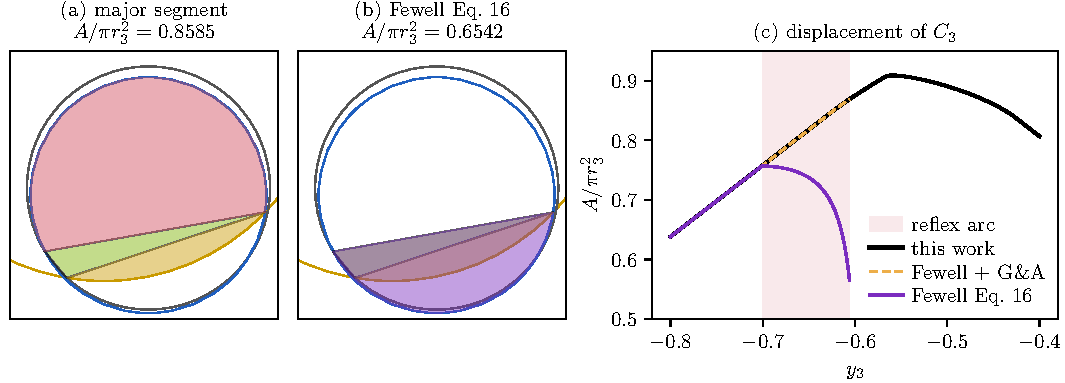
\includegraphics[width=\textwidth]{figures/reflex.pdf}
\caption{A circular triangle with an arc of $3.78$\,rad on the smallest
circle $C_3$. (a) Heron triangle and segments with the major segment on
$C_3$, which gives the exact area. (b) The segment of Fewell's Eq.~16,
which takes the minor arc. (c) Overlap area as $C_3$ moves along $y$:
the shaded interval contains a reflex arc.}
\label{fig:reflex}
\end{figure*}

\subsection{Public software} \label{sec:software}

We evaluated five public packages on the $40{,}000$ configurations of
Section~\ref{sec:accuracy}, of which $21{,}568$ have a non-zero overlap and
$18{,}432$ an empty one: \texttt{gefera} \citep[commit e27e832, compiled
from its Fortran source with its own flags and, with identical results,
with \texttt{-O2};][]{GordonAgol2022}, \texttt{eulerr} 7.1.0
\citep{eulerr}, \texttt{venn.js} \citep{vennjs}, \texttt{matplotlib-venn}
1.1.2 \citep{mplvenn} and Shapely 2.1.2 with GEOS 3.14.1
\citep{shapely, geos} at 8, 64 and 512 polygon segments per quarter
circle. \texttt{gefera} returns the flux of a star occulted by two bodies;
for a uniform source this is the area of the union of the two shadows on
the star, $|S\cap(P\cup M)|$, and we compare that quantity directly, which
spares \texttt{gefera} the cancellation of an inclusion--exclusion. We
count as a gross failure an undefined result, an exception, a relative
error above $10^{-3}$ for a non-empty overlap, or a non-zero result
exceeding $10^{-9}$ of the smallest disk for an empty one.
Table~\ref{tab:software} summarises the results.

\begin{deluxetable*}{lcccc}
\tablecaption{Public software on $40{,}000$ configurations\label{tab:software}}
\tablehead{
\colhead{Code} & \colhead{Undefined or exception} & \colhead{Wrong by $>10^{-3}$} & \colhead{Max.\ error$/\kappa u$} & \colhead{Median error$/\kappa u$}
}
\startdata
This work                         & 0    & 0     & 2.0                 & 0.12 \\
\texttt{gefera}, union area       & 31   & 90    & \nodata             & \nodata \\
\texttt{eulerr} 7.1.0             & 0    & 766   & $9.7\times10^{13}$  & 2.7 \\
\texttt{venn.js}                  & 0    & 3689  & $7.0\times10^{13}$  & 2.6 \\
\texttt{matplotlib-venn} 1.1.2    & 3746 & 1903  & $4.5\times10^{15}$  & 10 \\
Shapely, 8 segments               & 0    & 21568 & $7.0\times10^{14}$  & $1.1\times10^{13}$ \\
Shapely, 64 segments              & 0    & 11022 & $4.6\times10^{11}$  & $2.1\times10^{11}$ \\
Shapely, 512 segments             & 0    & 7294  & $7.1\times10^{9}$   & $3.5\times10^{9}$ \\
\enddata
\tablecomments{Errors relative to 50-digit references; $\kappa u$ as in
Table~\ref{tab:accuracy}. For \texttt{gefera} the union of the two
shadows on the star is compared, whose condition number differs from that
of the triple overlap; its maximum relative error is 0.95.}
\end{deluxetable*}

\texttt{gefera} computes the union to a median relative error of
$5\times10^{-16}$ and to $2.3\times10^{-10}$ in all hierarchical
configurations, but it returns undefined values in all 31 configurations
in which the disk of the planet lies inside that of the moon, and it
assigns wrong areas, with errors up to 95\%, to 90 circular
quadrilaterals, 88 of which involve a body larger than the star. It also
returns undefined values when a crossing of planet and moon lies exactly
on the limb and when $b+r=1$ for a single body. \texttt{eulerr} agrees
with the reference in general configurations but fails on 310 small
triangles and 448 thin lenses, and on 8 hierarchical configurations with
bodies of radius $0.02$ and $0.006$, where it returns either zero or the
full smallest disk in place of overlaps of 24 to 94\% of that disk.
\texttt{venn.js} fails on 1473 small triangles and 2216 thin lenses, with
relative errors up to $1.6\times10^{6}$: it evaluates circular segments
from their width with an arccosine of $1-w/r$ and tests containment with
an absolute tolerance of $10^{-10}$. \texttt{matplotlib-venn} raises an
exception in 3746 configurations in which one disk lies inside another,
because its region algebra excludes holes, returns zero in 886
configurations in which the smallest disk lies inside both others, and
fails on 1017 overlaps smaller than $5\times10^{-7}$ of the smallest
disk. Shapely is limited by its polygon resolution: with 512 segments per
quarter circle its median relative error is $1.9\times10^{-5}$, and small
and thin overlaps are lost entirely.

\subsection{Speed} \label{sec:speed}

We implemented the method in Python compiled with Numba \citep{Lam2015}
and timed batches of $2\times10^4$ configurations per topology on one core
of an Intel Core Ultra 5 226V, taking the best of nine repetitions.
The cost per configuration, including classification, translation and
evaluation, depends on the topology. The representative mixture of
all families costs 45\,ns, dominated by the early exits of empty and
contained configurations at 21--31\,ns; circular triangles cost
0.17\,$\mu$s and quadrilaterals 0.26\,$\mu$s. The specialised walks of
Section~\ref{sec:walk} halve the cost relative to the general walk, which
costs 117--427\,ns. The stable evaluation of Equations
(\ref{eq:area})--(\ref{eq:kahan}) costs the same as the direct
evaluation on the mixture and at most 41\% more on lenses. The closed form
of \citet{Fewell2006} with the correction of \citet{GordonAgol2022} costs
0.10\,$\mu$s for a circular triangle when the topology is known in
advance; it requires a case tree for all other configurations.

Table~\ref{tab:speed} and Figure~\ref{fig:speed} compare the public
packages on the same core, each
through its native interface, on the $40{,}000$ test configurations and on
two light-curve sequences of $2\times10^{5}$ positions of a planet and a
moon on the stellar disk with fixed radii. The present method is 4--5
times faster than \texttt{gefera}, 6 times faster than \texttt{venn.js},
and 80 to 5700 times faster than \texttt{eulerr}, \texttt{matplotlib-venn}
and Shapely.

\begin{deluxetable}{lccc}
\tablecaption{Cost per configuration in ns\label{tab:speed}}
\tablehead{
\colhead{Code} & \colhead{Test set} & \colhead{$r_p,r_m=0.1,0.0092$} & \colhead{$0.12,0.05$}
}
\startdata
This work (Numba)            & 82      & 47      & 99 \\
\texttt{gefera} (Fortran)    & \nodata & 202     & 514 \\
\texttt{venn.js} (Node.js)   & 465     & 265     & 573 \\
\texttt{eulerr} (R)          & 6825    & 5350    & 6550 \\
\texttt{matplotlib-venn}     & 30074   & 45667   & 86749 \\
Shapely, 8 segments          & 34761   & 35978   & 41859 \\
Shapely, 64 segments         & 83172   & 92478   & 103402 \\
Shapely, 512 segments        & 467650  & 907037  & 949028 \\
\enddata
\tablecomments{\texttt{gefera} accepts one pair of radii per call and is
timed on the sequences only; it evaluates its limb-darkening integrals
also for a uniform source. The \texttt{eulerr} times include 1.8\,$\mu$s of
R loop overhead per configuration; \texttt{venn.js} times include the
construction of its circle objects. The test set contains more triangles
than the mixture quoted in the text.}
\end{deluxetable}

\begin{figure}
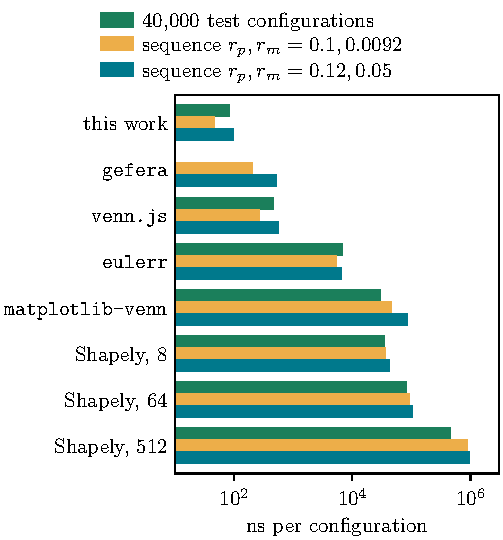
\includegraphics[width=\columnwidth]{figures/speed.pdf}
\caption{Cost per configuration on one CPU core (Table~\ref{tab:speed}),
logarithmic scale, for the $40{,}000$ test configurations and two
light-curve sequences of a planet and a moon with fixed radii.
\texttt{gefera} accepts one pair of radii per call and is timed on the
sequences only; Shapely is shown at 8, 64 and 512 segments per quarter
circle.}
\label{fig:speed}
\end{figure}

\section{Discussion} \label{sec:discussion}

The method separates topology from evaluation. The proposition reduces
the topology to the number of vertices, and the walk determines the
boundary without any formula that depends on the configuration. The
evaluation then applies one expression to every topology. This structure
removes the failure modes of earlier work at their origin: the reflex
error of \citet{Fewell2006} and \citet{Kipping2011} cannot occur because
no arc is inferred from a chord, and the precision loss of
Equation~(\ref{eq:lens}) cannot occur because no arccosine of an argument
near unity and no difference of nearly equal areas is formed. The
resulting algorithm is backward stable in the componentwise sense over
all tested geometries, including the near-tangent configurations that
arise at every ingress and egress of a mutual event. The failures of the
public packages in Section~\ref{sec:software} fall into the same two
classes: case trees that omit topologies, such as nested bodies and
quadrilaterals in \texttt{gefera} or holes in \texttt{matplotlib-venn},
and a loss of the small and thin overlaps of ingress and egress, which in
\texttt{venn.js} stems from its segment formula and absolute tolerance
and affects \texttt{eulerr} and \texttt{matplotlib-venn} alike.

The cost of the complete computation is that of a few square roots and
one arctangent per boundary arc. In a photodynamical model the
overlapping configurations form a small fraction of all samples, and most
evaluations end in the early exits at 21--31\,ns. The method therefore
removes the three-disk geometry as a computational concern from light-curve
models, and its error is bounded by the conditioning of the data.

The area and the centroid of the overlap determine the light blocked
twice during a mutual event to first order in the gradient of the stellar
intensity. The exact limb-darkened flux requires the line integrals of
\citet{Pal2012} and \citet{GordonAgol2022} along the same boundary arcs.
The walk of Section~\ref{sec:walk} supplies these arcs, their end points
and their orientation for every topology, and the stable crossings of
Equation~(\ref{eq:kahan}) supply accurate end points for the elliptic
integrals; the boundary walk thus serves as a robust front end for exact
mutual-transit photometry. The proposition and the walk extend without
change to disks of any relative size, including bodies larger than the
star in stellar triples.

\section{Conclusions} \label{sec:conclusion}

We have presented an exact solution for the area of the common overlap of
three disks that is complete, backward stable and fast. A proof that the
overlap has at most four corners reduces the geometry to five topologies
resolved by one boundary walk. Green's theorem, evaluated as circular
segments with series for thin segments, a vertex polygon relative to its
first vertex, and crossings from Kahan's stable triangle area, yields
errors below $2.01\,\kappa u$ for all $21{,}568$ tested configurations, where
the classical formulas err by factors up to $10^{16}$ of this bound or,
for reflex arcs, by up to 66\% of the area. Five public packages,
including the mutual-transit code \texttt{gefera}, fail on between 121
and $21{,}568$ of $40{,}000$ configurations; the present method fails on
none. The complete computation costs 45\,ns per configuration on average
and 0.26\,$\mu$s in the most complex topology, four to several thousand
times less than the public packages. The same decomposition gives the centroid of the overlap in
closed form. An open-source implementation is available at
\url{https://github.com/hippke/reuleaux}.

\begin{acknowledgments}
AI (Anthropic Claude Opus 5.5) was used to derive the solution and assist
the exposition of the text.
\end{acknowledgments}

\software{NumPy \citep{Harris2020}, Numba \citep{Lam2015}, mpmath
\citep{mpmath}, Matplotlib \citep{Hunter2007}, \texttt{gefera}
\citep{GordonAgol2022}, \texttt{eulerr} \citep{eulerr}, \texttt{venn.js}
\citep{vennjs}, \texttt{matplotlib-venn} \citep{mplvenn}, Shapely
\citep{shapely}, GEOS \citep{geos}}

\bibliography{references}{}
\bibliographystyle{aasjournalv7}

\end{document}
